\documentclass[11pt,a4paper]{article}
\usepackage[margin=25mm]{geometry}
\usepackage{indentfirst}
\usepackage{booktabs,tabularx,longtable}
\usepackage{tikz}
\usetikzlibrary{arrows.meta}
\usepackage[round,authoryear]{natbib}
\usepackage[hidelinks]{hyperref}
\usepackage{amsmath,graphicx,url,placeins}
\usepackage{microtype,needspace}
\setlength{\parskip}{6pt}
\renewcommand{\topfraction}{0.9}
\renewcommand{\textfraction}{0.1}
\renewcommand{\floatpagefraction}{0.9}

\title{From Correlation to Causation: Recovering Causal Structure in Psychological Networks}
\author{Harsh Nagouda - 1893580\\ \small BEP partial thesis draft}
\date{9 November 2026}
\begin{document}
\maketitle

\section{Introduction}
Psychological symptoms often occur together. For example, people who sleep poorly may also report feeling tired. A psychological network shows these relationships. Each symptom is a point, called a \emph{node}, and a line between two symptoms is an \emph{edge}.

A connection does not establish what causes what. Poor sleep might cause tiredness, but a third factor might also affect both. This matters when using a network to decide which symptom to treat. Knowing that two symptoms are related is different from knowing what would happen if one of them were changed.

This thesis asks how much can be learned about cause and effect from the psychological datasets collected in ReBayesed. These are cross-sectional datasets: they do not follow changes in symptoms over time. The algorithm used in an attempt to recover causal structures is the Peter-Clark (PC) algorithm, which can help find connections and assess which directions the data can support, under a set of assumptions \citep{spirtes1993,kalisch2007}.

\subsection{The research problem}
The networks studied here (and those used in the ReBayesed project) are Gaussian graphical models. In these models, an edge represents a \emph{partial correlation}: a relationship between two symptoms after taking the other measured symptoms into account \citep{borsboom2013}.

PC asks a different question. It checks whether two variables become statistically independent when other variables are taken into account. It uses these checks to narrow down the possible causal structures. Several structures may still fit the same evidence, leaving some directions unresolved.

Figure~\ref{fig:edges} distinguishes a partial-correlation edge from the two edge types used in the PC output. The same plain line has a different meaning in the two graph types: an association in the original network, and an unresolved direction in the causal equivalence class.

\begin{figure}[!htbp]
\centering
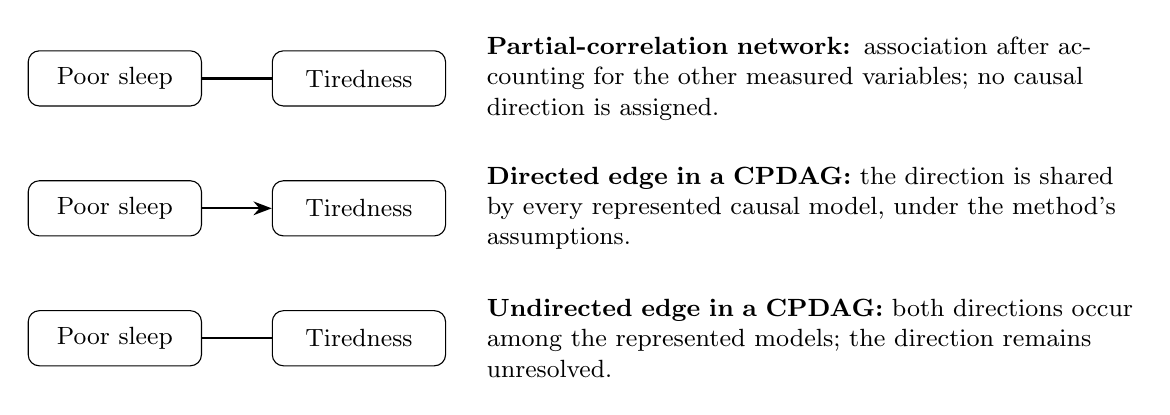
\begin{tikzpicture}[>=Stealth, every node/.style={font=\small}, symptom/.style={draw,rounded corners,minimum width=22mm,minimum height=7mm}, meaning/.style={anchor=west,text width=82mm}]
\node[symptom] (a) at (0,0) {Poor sleep};
\node[symptom] (b) at (3.1,0) {Tiredness};
\draw[thick] (a)--(b);
\node[meaning] at (4.6,0) {\textbf{Partial-correlation network:} association after accounting for the other measured variables; no causal direction is assigned.};
\node[symptom] (c) at (0,-1.65) {Poor sleep};
\node[symptom] (d) at (3.1,-1.65) {Tiredness};
\draw[thick,->] (c)--(d);
\node[meaning] at (4.6,-1.65) {\textbf{Directed edge in a CPDAG:} the direction is shared by every represented causal model, under the method's assumptions.};
\node[symptom] (e) at (0,-3.3) {Poor sleep};
\node[symptom] (f) at (3.1,-3.3) {Tiredness};
\draw[thick] (e)--(f);
\node[meaning] at (4.6,-3.3) {\textbf{Undirected edge in a CPDAG:} both directions occur among the represented models; the direction remains unresolved.};
\end{tikzpicture}
\caption{An introductory guide to edge meanings. CPDAG stands for completed partially directed acyclic graph and is explained in Section~\ref{sec:pc-method}. The symptoms are illustrative, rather than an empirical result. An undirected CPDAG edge does not indicate a feedback loop.}
\label{fig:edges}
\end{figure}
\FloatBarrier

PC starts from each dataset's correlation matrix, a table showing the correlations between its variables. It learns its own connections and directions. It does not take the published network and simply add arrows to its existing edges.

\subsection{Why this question matters}
In the ReBayesed project, \citet{huth2026} re-analysed 293 psychological networks from 126 papers. They used Bayesian model averaging to assess the evidence for connections without assigning causal directions. Bayesian model averaging combines evidence across possible models instead of relying on just one model.

Their work raises a further question: if the data provide clearer evidence that symptoms are connected, do they also provide clearer evidence about the direction of those connections? These are separate questions. Strong evidence for a connection does not necessarily establish its direction.

The hypothesis for the first research question is that networks with more observations per possible edge have a larger share of edges with a direction. An observation here usually means one participant. If this pattern exists, it could help guide later work on how much data a study needs.

However, a larger sample cannot settle every question about direction. Different causal structures can produce the same pattern of statistical independence. The analysis must therefore distinguish between uncertainty caused by limited data and uncertainty that more data cannot resolve.

\subsection{Related work}
\citet{huber2024} explains why observational data can leave several causal structures equally possible. This problem becomes more difficult when an unmeasured factor affects two or more measured variables. The paper also explains the assumptions needed to interpret a graph causally; the assumptions used here are listed in Section~\ref{sec:pc-method}. An arrow returned by a program is not enough on its own.

A simple example uses three variables: poor sleep ($A$), tiredness ($B$) and concentration problems ($C$). Figure~\ref{fig:equivalence} shows three possible causal structures. Under the Markov and faithfulness assumptions, all three imply the same pattern: $A$ and $C$ are associated, but become independent after accounting for $B$. Conditional-independence evidence alone therefore cannot distinguish these structures, even with unlimited data. This is a schematic example, rather than a claim about the actual causes of these symptoms \citep{huber2024,spirtes1993}.

\begin{figure}[!htbp]
\centering
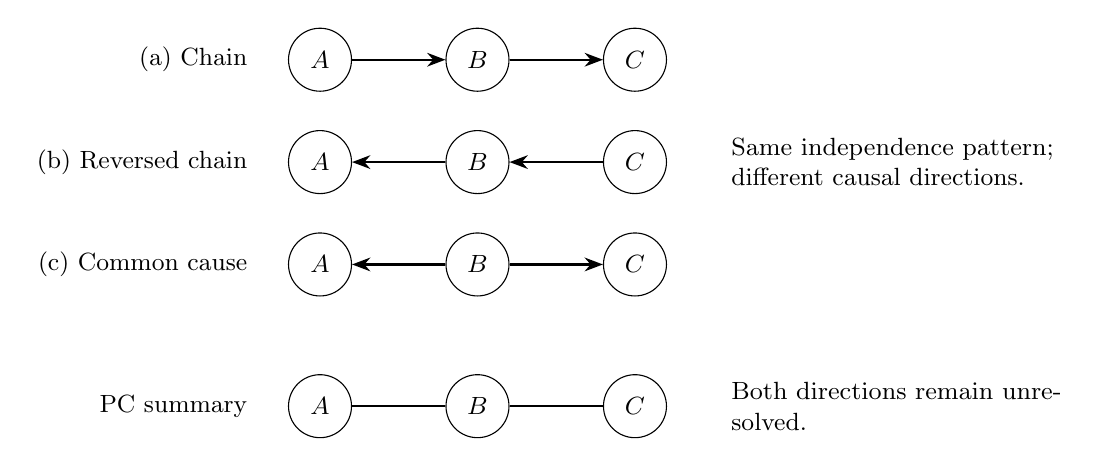
\begin{tikzpicture}[>=Stealth,varnode/.style={circle,draw,minimum size=8mm},every node/.style={font=\small}]
\foreach \y/\lab in {0/{(a) Chain},-1.3/{(b) Reversed chain},-2.6/{(c) Common cause}} {
  \node[anchor=east] at (-0.8,\y) {\lab};
}
\node[varnode] (a1) at (0,0) {$A$}; \node[varnode] (b1) at (2,0) {$B$}; \node[varnode] (c1) at (4,0) {$C$};
\draw[thick,->] (a1)--(b1); \draw[thick,->] (b1)--(c1);
\node[varnode] (a2) at (0,-1.3) {$A$}; \node[varnode] (b2) at (2,-1.3) {$B$}; \node[varnode] (c2) at (4,-1.3) {$C$};
\draw[thick,->] (c2)--(b2); \draw[thick,->] (b2)--(a2);
\node[varnode] (a3) at (0,-2.6) {$A$}; \node[varnode] (b3) at (2,-2.6) {$B$}; \node[varnode] (c3) at (4,-2.6) {$C$};
\draw[thick,->] (b3)--(a3); \draw[thick,->] (b3)--(c3);
\node[anchor=west,align=left,text width=43mm] at (5.1,-1.3) {Same independence pattern; different causal directions.};
\node[varnode] (a4) at (0,-4.4) {$A$}; \node[varnode] (b4) at (2,-4.4) {$B$}; \node[varnode] (c4) at (4,-4.4) {$C$};
\draw[thick] (a4)--(b4); \draw[thick] (b4)--(c4);
\node[anchor=east] at (-0.8,-4.4) {PC summary};
\node[anchor=west,align=left,text width=43mm] at (5.1,-4.4) {Both directions remain unresolved.};
\end{tikzpicture}
\caption{Three causal structures in the same Markov equivalence class and their undirected CPDAG summary. Here, $A$ is poor sleep, $B$ is tiredness and $C$ is concentration problems. In contrast, $A\to B\leftarrow C$ is a collider and implies a different independence pattern, so it is not part of this class.}
\label{fig:equivalence}
\end{figure}
\FloatBarrier

For analysis, the R package \texttt{pcalg} is used, which can work directly with a correlation matrix and sample size \citep{kalisch2012}. Its PC-stable option makes the estimated set of connections independent of the order in which variables are listed \citep{colombo2014}. This set of connections, without arrow directions, is called the \emph{skeleton}. A limitation of PC-stable however, is that it does not guarantee that the later step of assigning directions is also independent of variable order — which is discussed as part of research question 1. 

\subsection{Research questions and scope}
The central goal is to explore \textbf{how much can be learned about causal structure from the ReBayesed psychological datasets, and what limits that learning?}

The thesis addresses three research questions:
\begin{enumerate}
\item \textbf{RQ1}: Do networks with more observations per possible edge have a larger share of retained edges with a direction?
\item \textbf{RQ2}: Is stronger Bayesian evidence for connections associated with a larger share of edges with a direction?
\item \textbf{RQ3}: How do the conclusions change when the method allows for unmeasured common causes?
\end{enumerate}

This partial draft reports the methods and completed results for RQ1, including checks using different test thresholds and variable orders. The main analysis uses one network per paper. Other networks are analysed separately.

RQ2, the comparison with Fast Causal Inference (FCI) for RQ3, and comparisons between studies measuring the same symptoms are still planned. Section~\ref{sec:outline} explains the remaining work.

\section{Data}
\subsection{Where the data come from}
The input is the ReBayesed application export, \path{filtered-network-data-2026-09-21.rds}. It contains correlation matrices, reported sample sizes and information about the studies. It does not contain individual participants' responses. The R analysis reads these summary statistics directly, so it does not need reconstructed responses or synthetic data.

The export contains 294 networks, while the article reports 293. Network \texttt{N0423\_2} was removed as it was an extra network found by comparing the export with the authors' results copy on the Open Science Framework (OSF). This leaves 293 networks from 126 papers.

Although network \texttt{N0423\_2} is labelled ``Subset of variables'', it has the same 67 nodes as \texttt{N0423\_1}. Its reported sample size is 829 rather than 840. This does not settle every question about which networks appeared in the article. For example, the collection of cleaning scripts has no script for \texttt{N0986\_1}. Matching the results copy therefore does not independently confirm the article's exact set of networks.

RQ1 includes all 293 remaining networks, with no restriction to a topic or questionnaire. Depression networks were used to test the pipeline at the start, but the main analysis covers the full collection.

Reported sample sizes range from 23 to 388,286, and networks contain between 3 and 86 variables. The study information classifies 71 networks as continuous, 195 as ordinal and 27 as mixed. Continuous variables can take values along a scale. Ordinal variables use ordered categories, such as questionnaire ratings from ``never'' to ``always''. Mixed networks contain both types.

Every network has a sample size and a correlation matrix containing only finite values. The required inputs are therefore available for all networks. This does not mean that all networks meet the assumptions of the statistical test, especially those with ordinal variables.

\subsection{Why use correlation matrices?}
Individual participant data would allow more checks and alternative methods. For example, it would allow resampling of participants, checking of the exported correlations, or use methods based on ranks to handle ordinal responses. These methods would provide alternatives to treating category scores as continuous measurements.

However, limiting the study to networks with participant data would substantially change the sample. Only 62 of the 293 networks, from 30 papers, have a recorded data link. A link also does not guarantee that the data can actually be retrieved.

None of the 36 networks tagged as depression has a data link. Networks with links also cover different topics: 24\% have the Clinical tag, compared with 57\% of networks without links. A study restricted to these links would therefore cover a different part of the collection. It would also leave no depression networks for the planned comparison of matching symptoms.

Using the correlation matrices and reported sample sizes gives all 293 networks the same type of input. It also means accepting the limits of working without participant responses.

\subsection{Selecting one network per paper}
Of the 126 papers, 57 contribute more than one network. Networks from the same paper may share participants or differ only in which variables or models were used. Counting every network as an independent study would give these papers more weight and could make a pattern look better supported than it is.

The main analysis therefore uses one randomly selected network per paper, giving 126 networks. Network IDs are sorted before selection. A fixed random seed of 2026 makes the choice repeatable. Selection happens before PC is run and does not depend on its results. Appendix~\ref{app:selection} lists all 126 chosen networks and their paper IDs.

The remaining 167 networks are analysed separately. They provide additional descriptions, but they are not independent replications of the main analysis.

\subsection{Keeping track of variable names}
Each matrix keeps the variable order from the export. PC uses node numbers internally, and a separate CSV file stores the original matrix labels. This lets the analysis run when a label is missing without changing the correlations or inventing a symptom name.

The labels come from the matrices because the metadata field \texttt{variable\_names} can list names in a different order. Pairing that list with matrix columns by position could give a variable the wrong name. As a sanity check, network \texttt{N0029\_1}'s cleaning script was checked to verify that the matrix labels match the final renamed columns. That check confirms the labels' origin in this example. However, it does not establish that labels match across all studies.

Symptom names have not yet been matched across studies. The current analysis therefore does not compare directions for a shared set of symptoms. Selecting one network per paper also keeps identical inputs from the same paper from appearing together in the main sample. Such duplicates can remain among the additional networks, which are not treated as independent observations.

\section{Methods and approach}
\subsection{How PC uses the data}\label{sec:pc-method}
\texttt{pcalg::pc()} with \texttt{gaussCItest}, a Gaussian Fisher-z test for conditional independence \citep{kalisch2012} is run. Conditional independence means that two variables become statistically independent after taking a specified set of other variables into account. Each network supplies its correlation matrix and reported sample size as \texttt{list(C = correlation, n = sample\_size)}.

PC uses these tests to estimate which variables are connected and which directions can be assigned. Under its assumptions (discussed below), the intended output is a \emph{completed partially directed acyclic graph}, or CPDAG. This graph represents a group of causal models that imply the same conditional independencies. That group is called a \emph{Markov equivalence class}.

In a CPDAG, a directed edge has the same direction in every model in that group. An undirected edge means that the direction is still unresolved. The models represented by a CPDAG are directed acyclic graphs (DAGs): they have arrows but no path of arrows that loops back to its starting point.

\Needspace{8\baselineskip}
Reading these arrows as causal requires several assumptions:
\begin{itemize}
\item \textbf{Acyclicity:} the causal system has no feedback loops.
\item \textbf{Causal sufficiency:} there are no unmeasured common causes of the measured variables.
\item \textbf{The Markov condition:} the causal graph correctly implies certain statistical independencies in the data.
\item \textbf{Faithfulness:} statistical independencies reflect the graph's structure, rather than effects that happen to cancel each other out.
\end{itemize}

A graph can have the required mathematical structure even when these assumptions do not hold in the real system.

The exported matrices contain Pearson correlations. The source cleaning workflow calculated them using \texttt{cor(na.omit(data))}, which removes rows with missing values before calculating correlations. Keeping these matrices gives this analysis the same input basis as the ReBayesed Gaussian graphical models and the planned Bayesian comparison. However, most networks contain ordinal or mixed variables. Using a Gaussian test for these data remains a limitation.

\subsection{Test thresholds and graph settings}
The baseline sets a significance threshold of $\alpha=0.01$ for each conditional-independence test. This threshold helps determine whether PC keeps or removes a connection.

The decision log bases this starting point on simulations in \citet{kalisch2007}. In those simulations, the average structural Hamming distance, a measure of graph errors, was lowest around $\alpha=0.005$--$0.01$. This does not show that the same threshold is best for this varied collection of psychological datasets and therefore, thresholds of $0.001$ and $0.05$ are also tested. 

The option \texttt{skel.method = "stable"} uses PC-stable. It removes variable-order effects from the estimated skeleton, but directions can still depend on that order \citep{colombo2014}. The baseline uses the exported variable order. It adds no prior restrictions on edges and sets no explicit limit on how many variables a test can condition on.

The option \texttt{u2pd = "relaxed"} keeps the output even when it is not a valid CPDAG. This avoids replacing an unresolved graph with a single arbitrarily chosen DAG. The conservative PC, majority-rule PC and conflict-handling options remain at their defaults: all are false \citep{pcalgpc}.

Each returned graph is checked with \texttt{isValidGraph(type = "cpdag")} and both the result and any messages are saved \citep{pcalgvalid}. Fitting errors are also recorded. A run that finishes is therefore distinguished from a run that returns a valid graph.

\subsection{Measuring data volume and the share of arrows}
RQ1 compares two quantities. The first is the number of observations per possible edge, called \emph{data volume} here. With $p$ variables, there are
\begin{equation}
M=\frac{p(p-1)}{2}
\end{equation}
possible edges. If the sample size is $n$, data volume is $V=n/M$.

For example, nine variables give 36 possible edges. With 1,610 observations, data volume is $1610/36=44.722$. The denominator counts every possible edge, including those PC removes. It therefore does not depend on the graph PC returns.

The second quantity is the \emph{arrow fraction}: the share of retained edges that have a direction. A retained edge is any connection left by PC. If $D$ edges are directed and $U$ are undirected, then
\begin{equation}
F=\frac{D}{D+U}.
\end{equation}
For example, if PC keeps ten connections and six have arrows, the arrow fraction is $0.6$, or 60\%. Each pair of nodes is counted once. If PC keeps no edges, the fraction is undefined, because there are no connections to assess.

Edge counts are saved for every completed run. The arrow fraction is interpreted as a summary of resolved directions only when the graph passes the CPDAG check.

\subsection{Comparing the two measures}
The analysis plots (Figure 3) data volume against arrow fraction for valid graphs with at least one edge. The horizontal axis uses a logarithmic scale because data volume varies widely. On this scale, equal distances represent equal ratios rather than equal differences.

Spearman's rank correlation summarises whether networks with larger data volumes tend to have larger arrow fractions. A value near $1$ indicates an increasing pattern, a value near $-1$ a decreasing pattern, and a value near zero little or no consistent increasing or decreasing pattern. It does not measure causal accuracy.

The main sample and additional networks are summarised separately. No inferential p-value is reported, and the additional networks are not pooled as independent studies. Fitting errors, invalid graphs and the ranges before and after restricting the analysis to valid graphs are also reported. This shows how much of the original sample enters the comparison.

Sample size has another role: PC uses it in its statistical tests. For a fixed partial correlation $r_{ij\mid S}$ between variables $i$ and $j$, after accounting for variables in set $S$, the Fisher-z statistic is
\begin{equation}
Z_{ij\mid S}=\sqrt{n-|S|-3}\;\operatorname{atanh}(r_{ij\mid S}).
\end{equation}

Here, $|S|$ is the number of variables being accounted for, and $\operatorname{atanh}$ transforms the correlation for the test. At $\alpha=0.01$, the test rejects independence when $|Z_{ij\mid S}|$ is greater than about $2.576$.

With no other variables accounted for, the required absolute correlation is about $0.52$ at $n=23$, but only $0.004$ at $n=388{,}286$. Accounting for more variables raises the required correlation. A fixed significance threshold therefore does not mean that the same correlation is needed in every network. Therefore, any relationship between data volume and arrow fraction must be read with this in mind. 

Networks also differ in their number of variables and in what they measure. The comparison cannot show what would happen if the sample size of the same study were increased.

\subsection{Checking thresholds and variable order}
The sensitivity checks use the same 126 networks as the main analysis and change one setting at a time. Two runs change $\alpha$ to $0.001$ and $0.05$ while keeping the original variable order. Three other runs keep $\alpha=0.01$ and shuffle the variable order using seeds 2027, 2028 and 2029. These thresholds and seeds were fixed before inspecting the sensitivity results. The additional 167 networks are not rerun.

Each shuffle applies the same permutation to the rows and columns of a correlation matrix. It changes where variables appear without changing their correlations. Original node numbers stay attached as labels. After fitting, the graph is put back into the original order so that corresponding variables can be compared. Three shuffles provide a repeatable check, but do not test every possible order. All other settings stay the same.

For each run, the recorded summaries include the number of valid graphs, arrow fractions, Spearman correlation and changes in individual graphs. A changed node pair means that a connection was added, removed or given a different direction. A changed skeleton pair means only that a connection was added or removed.

These graph comparisons intentionally include invalid outputs to accurately describe what the program returned. Two graphs can have the same number of arrows while assigning different directions to individual edges — an unchanged arrow fraction therefore does not guarantee unchanged directions.

Changing a setting can affect which networks produce usable graphs. Each changed run is therefore compared with the baseline using only networks that are usable in both. This keeps the comparison fair. For each shared network, the analysis checks whether the proportion of edges with arrows changed. It uses the edge counts directly, so rounding cannot make two equal proportions appear different.

\subsection{Implementation and checks}
The R script \path{R/rq1.R} selects the main sample, fits PC and saves correlation matrices, node labels, adjacency matrices and per-network results as CSV files. An adjacency matrix records which node pairs are connected and in which direction. The Python module \path{src/bep/rq1.py} summarises the main and additional samples separately.

The saved session uses R 4.6.2 and \texttt{pcalg} 2.7-12. R package versions are recorded through \texttt{renv}. The sensitivity scripts are \path{R/rq1_sensitivity.R} and \path{src/bep/rq1_sensitivity.py}.

All 630 sensitivity outputs were checked for matrix dimensions, entries of zero or one, edge counts and fractions. All three shuffle sequences were reproduced from their seeds. After putting variables back in their original order, every shuffled skeleton matched the baseline. Summaries for the shared valid networks also agreed with the per-network comparisons. These checks show that the saved results are consistent with the pipeline. They do not test whether its causal assumptions hold.

\section{RQ1 results}\label{sec:results}
\subsection{How many outputs could be used?}
All 126 networks from the main sample finished without fitting errors. However, only 25, or 19.8\% graphs passed the CPDAG check. One of those had no edges, leaving 24 graphs for the RQ1 comparison. The other 101 outputs failed the check.

All 167 additional networks also finished. Of these, 47 were valid CPDAGs. Nine had no edges, leaving 38 for the separate comparison (Table~\ref{tab:counts}). These additional networks come from 57 papers already represented in the main sample.

\begin{table}[!htbp]
\centering
\caption{Completed runs and graph validity. The comparison uses only valid graphs with at least one edge. Validity percentages use completed fits as the denominator.}
\label{tab:counts}
\begin{tabular}{@{}lrr@{}}
\toprule
 & Main sample & Additional networks\\
\midrule
Selected networks & 126 & 167\\
Completed fits & 126 & 167\\
Fitting errors & 0 & 0\\
Valid CPDAGs & 25 & 47\\
Invalid outputs & 101 & 120\\
Valid graphs with at least one edge & 24 & 38\\
\bottomrule
\end{tabular}
\end{table}
Finishing a run therefore does not mean that its output has the graph structure needed for the intended interpretation.

\FloatBarrier
\subsection{Data volume and arrow fraction}
Among the 24 usable graphs in the main sample, data volume ranges from $0.320$ to $192.500$ observations per possible edge. Arrow fraction ranges from $0.000$ to $1.000$. Spearman's correlation is $\rho=0.005$ (Figure~\ref{fig:rq1}). There is almost no consistent increasing or decreasing pattern in these 24 graphs.

\begin{figure}[!htbp]
\centering
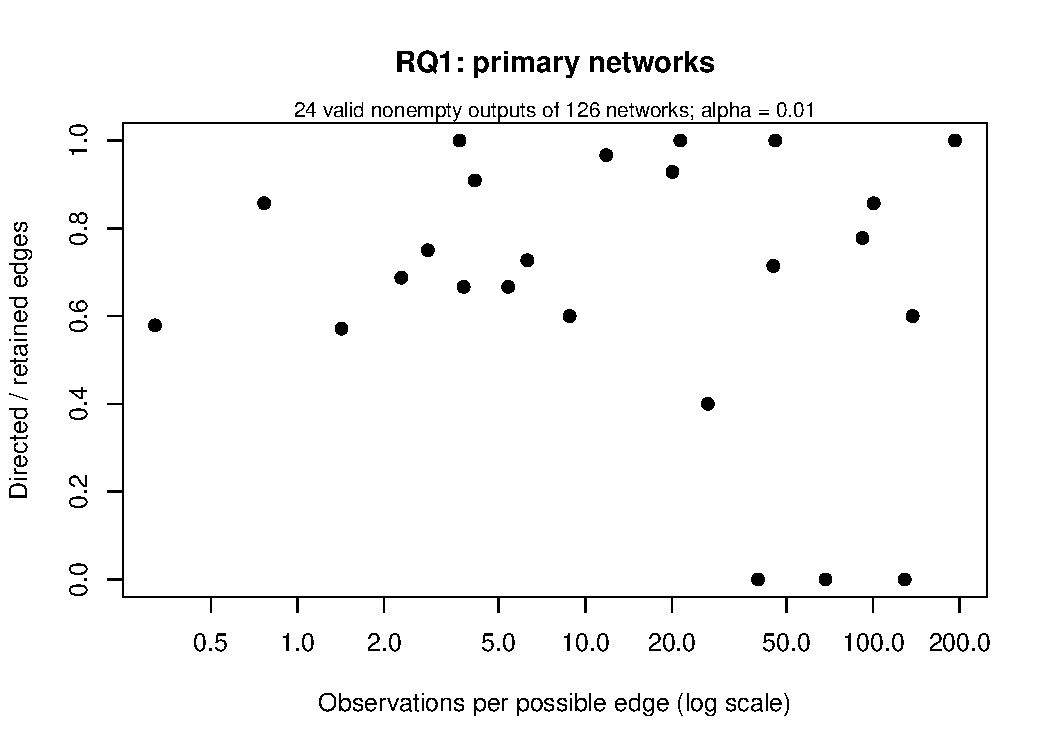
\includegraphics[width=0.82\textwidth]{figures/primary_rq1.pdf}
\caption{Data volume and arrow fraction for the 24 valid graphs with at least one edge in the main sample. The original selection contains 126 networks, one per paper, chosen using seed 2026. The horizontal axis is logarithmic. Table~\ref{tab:counts} reports outputs excluded from this plot.}
\label{fig:rq1}
\end{figure}

The usable graphs cover a narrower range than the full main sample. Across all 126 selected networks, sample sizes range from 30 to 388,286 and node counts from 3 to 76. In the 24 plotted networks, sample sizes range from 64 to 2,057 and node counts from 3 to 25. Data volume in the full main sample ranges from $0.189$ to $7{,}059.745$.

The near-zero correlation therefore describes a small, selected part of the main sample. It cannot be assumed to describe all 126 networks.

For the additional networks, the correlation is $\rho=-0.258$, based on 38 valid graphs with edges. This is a descriptive result. These networks can share participants, and papers contribute different numbers of networks. It is not an independent replication of the main result.

\subsection{What changed in the sensitivity checks?}
All five sensitivity runs used the same 126 selected networks. All 630 fits finished without fitting errors. Table~\ref{tab:sensitivity} shows how many graphs could be used and the correlation for each run.

\begin{table}[!htbp]
\centering
\caption{Sensitivity checks for the fixed main sample. Each correlation uses that run's valid graphs with at least one edge, so different rows can describe different subsets of networks.}
\label{tab:sensitivity}
\begin{tabular}{@{}lrrr@{}}
\toprule
Run & Valid CPDAGs & With edges & Spearman $\rho$\\
\midrule
Baseline: $\alpha=0.01$ & 25 & 24 & 0.005\\
$\alpha=0.001$ & 22 & 21 & -0.091\\
$\alpha=0.05$ & 18 & 18 & -0.144\\
Order seed 2027 & 27 & 26 & -0.173\\
Order seed 2028 & 23 & 22 & -0.129\\
Order seed 2029 & 22 & 21 & -0.094\\
\bottomrule
\end{tabular}
\end{table}

Neither alternative threshold shows the expected positive pattern in its usable subset. At $\alpha=0.001$, 21 graphs give $\rho=-0.091$. At $\alpha=0.05$, 18 give $\rho=-0.144$.

Interestingly however, the subsets change. Only 14 networks are usable in both the baseline and the $0.001$ run. For these same 14 networks, the baseline correlation is $-0.071$ and the variant correlation is $0.033$. Only 11 networks are usable in both the baseline and the $0.05$ run. Their correlations are $-0.037$ and $-0.078$, respectively. Changing the threshold therefore changes both the graphs and which networks enter the comparison.

Shuffling variable order leaves every network's skeleton unchanged. Even so, the full returned graph differs from the baseline in 112, 118 and 116 of the 126 networks for seeds 2027, 2028 and 2029. These counts include invalid graphs and describe changes in the directions returned by the software.

The shuffled runs leave 26, 22 and 21 usable graphs, with correlations of $-0.173$, $-0.129$ and $-0.094$. The same connections can therefore lead to different directions or different validity outcomes.

The correlations above use all usable networks in each run, so they can change partly because different networks pass validation. To compare results on the same networks, each shuffled run is also paired with the baseline using only networks whose graphs are valid and contain at least one edge in both runs. Table~\ref{tab:shared-shuffles} reports these three separate comparisons. Each row uses its own overlapping set of networks; the sets are not necessarily identical across rows.

\begin{table}[!htbp]
\centering
\small
\caption{Baseline and shuffled results compared on the same networks. Both Spearman correlations in a row relate data volume to arrow fraction using only that row's shared networks. The final column is the absolute difference between the two correlations, calculated before rounding.}
\label{tab:shared-shuffles}
\begin{tabular}{@{}lrrrrr@{}}
\toprule
Shuffle seed & Shared networks & Fraction changed & Baseline $\rho$ & Shuffled $\rho$ & $|\Delta\rho|$\\
\midrule
2027 & 16 & 5 & 0.001 & 0.039 & 0.037\\
2028 & 13 & 4 & -0.114 & -0.122 & 0.008\\
2029 & 13 & 3 & -0.036 & -0.033 & 0.003\\
\bottomrule
\end{tabular}
\end{table}

For example, 16 networks are usable in both the baseline and the seed-2027 run. Five of those 16 have a different arrow fraction after shuffling. Recalculating the data-volume--arrow-fraction correlation on those same 16 networks gives $\rho=0.001$ for the baseline and $\rho=0.039$ after shuffling, an absolute change of $0.037$ before rounding. These baseline correlations differ from the overall baseline value of $0.005$ because they use smaller subsets of its 24 usable networks. Small changes in these summary correlations do not imply that individual edge directions are stable.
\FloatBarrier

The overall correlations thus reflect both changes within networks and changes in which networks pass validation. These checks describe the software's output. They do not establish causal accuracy or solve the problem of excluding invalid graphs.

\FloatBarrier
\section{Discussion}
The main analysis does not show the expected positive relationship between observations per possible edge and the share of edges with a direction. However, this result is based on only 24 usable graphs, and the presence of 101 invalid outputs prevent a conclusion that the relationship is absent across the full main sample.

The sensitivity checks show why both graph changes and changes in the usable sample matter. Shuffling variable order leaves all connections unchanged, but can change directions and whether a graph passes validation. Changing the test threshold affects both the graphs and which networks can be compared.

None of the tested settings shows a clear positive rank correlation within its usable subset. This does not mean that the directions are unaffected by those choices.

\subsection{What these results can and cannot establish}
A high arrow fraction means that the returned graph assigns directions to many of its connections, but it does not show that those directions are correct.

The CPDAG check asks whether the output has the required graph structure. Causal interpretation also needs assumptions about how the data were generated. A failed check does not mean every arrow is false, and a passed check does not mean every arrow is correct. These validity rates apply to the tests and settings used here.

Another major limitation is that there is no known true causal graph for these datasets. Neither arrow fraction nor structural validity can therefore measure true causal accuracy.

\subsection{Unresolved problems and limitations}
The analysis has not established why so many outputs fail validation. The active pipeline uses the standard validity check. It does not rebuild failed graphs or investigate cycles in detail.

Studies analyzed in the ReBayesed project also use different questionnaires and sets of variables. Their arrow fractions therefore do not describe directions for a common set of symptoms. Choosing one network per paper reduces dependence between networks from the same paper, but does not guarantee that different papers used separate participant samples.

\section{Remaining work}\label{sec:outline}
RQ1 provides the first completed results chapter. The following sections describe planned analyses, followed by a final discussion and conclusion.

\subsection{Bayesian evidence for connections}
RQ2 will ask whether stronger Bayesian evidence for a connection is associated with a larger share of edges with a direction. This will be an exploratory comparison. Evidence that a connection exists may not provide the independence information needed to determine its direction.

The Bayesian probabilities also depend on a randomised search through a subset of possible networks. They should therefore be interpreted with that search process in mind.

\subsection{Allowing for unmeasured common causes}
RQ3 will compare PC with Fast Causal Inference (FCI), which allows for unmeasured common causes. This will show how the conclusions change when that possibility is allowed.

\subsection{Comparing studies that measure the same symptoms}
Comparing individual directions across studies first requires a mapping from matrix labels to shared symptom concepts. This is because different questionnaires present similar options albeit with different wording. For example, `Sleep' vs `SLEEP' vs `sleep\_problems' vs `I have trouble sleeping at night' depending on the paper. 

DSM-5 categories could help compare different questionnaires, but several items might map to one symptom. Questionnaire-specific items keep those differences visible, but limit which studies can be compared. 

\subsection{Final discussion and conclusion}
The final discussion will bring the research questions together. It will assess which uncertainties may reflect limited information and which come from different causal structures fitting the same evidence. It will also assess whether the methods support consistent conclusions under their different assumptions.

\clearpage
\appendix
\clearpage
\section{Networks selected for the main analysis}\label{app:selection}
Table~\ref{tab:selection} lists the fixed selection of 126 networks, one per paper, used for the baseline RQ1 analysis and all sensitivity checks. The IDs reproduce the saved selection generated with seed 2026. Inclusion in this table does not mean that the returned graph passed validation; Section~\ref{sec:results} reports those outcomes. The three pairs of columns continue the same list across each row.

\begingroup
\small
\setlength{\tabcolsep}{9pt}
\begin{longtable}{@{}llllll@{}}
\caption{Selected network IDs and their corresponding paper IDs.}\label{tab:selection}\\
\toprule
Network ID & Paper ID & Network ID & Paper ID & Network ID & Paper ID\\
\midrule
\endfirsthead
\caption[]{Selected networks and paper IDs (continued).}\\
\toprule
Network ID & Paper ID & Network ID & Paper ID & Network ID & Paper ID\\
\midrule
\endhead
\midrule
\multicolumn{6}{r}{Continued on the next page}\\
\endfoot
\bottomrule
\endlastfoot
\texttt{N0025\_1} & \texttt{N0025} & \texttt{N0029\_1} & \texttt{N0029} & \texttt{N0030\_1} & \texttt{N0030} \\
\texttt{N0050\_1} & \texttt{N0050} & \texttt{N0051\_1} & \texttt{N0051} & \texttt{N0059\_1} & \texttt{N0059} \\
\texttt{N0092\_1} & \texttt{N0092} & \texttt{N0105\_2} & \texttt{N0105} & \texttt{N0106\_1} & \texttt{N0106} \\
\texttt{N0122\_2} & \texttt{N0122} & \texttt{N0123\_1} & \texttt{N0123} & \texttt{N0164\_4} & \texttt{N0164} \\
\texttt{N0165\_1} & \texttt{N0165} & \texttt{N0166\_1} & \texttt{N0166} & \texttt{N0203\_1} & \texttt{N0203} \\
\texttt{N0262\_3} & \texttt{N0262} & \texttt{N0271\_1} & \texttt{N0271} & \texttt{N0293\_1} & \texttt{N0293} \\
\texttt{N0304\_2} & \texttt{N0304} & \texttt{N0306\_1} & \texttt{N0306} & \texttt{N0316\_4} & \texttt{N0316} \\
\texttt{N0318\_1} & \texttt{N0318} & \texttt{N0320\_1} & \texttt{N0320} & \texttt{N0327\_1} & \texttt{N0327} \\
\texttt{N0328\_1} & \texttt{N0328} & \texttt{N0332\_2} & \texttt{N0332} & \texttt{N0342\_1} & \texttt{N0342} \\
\texttt{N0376\_1} & \texttt{N0376} & \texttt{N0378\_4} & \texttt{N0378} & \texttt{N0380\_8} & \texttt{N0380} \\
\texttt{N0414\_1} & \texttt{N0414} & \texttt{N0423\_1} & \texttt{N0423} & \texttt{N0425\_3} & \texttt{N0425} \\
\texttt{N0431\_1} & \texttt{N0431} & \texttt{N0438\_3} & \texttt{N0438} & \texttt{N0440\_1} & \texttt{N0440} \\
\texttt{N0441\_2} & \texttt{N0441} & \texttt{N0442\_1} & \texttt{N0442} & \texttt{N0445\_1} & \texttt{N0445} \\
\texttt{N0448\_1} & \texttt{N0448} & \texttt{N0449\_2} & \texttt{N0449} & \texttt{N0450\_1} & \texttt{N0450} \\
\texttt{N0451\_1} & \texttt{N0451} & \texttt{N0455\_2} & \texttt{N0455} & \texttt{N0480\_7} & \texttt{N0480} \\
\texttt{N0493\_1} & \texttt{N0493} & \texttt{N0520\_1} & \texttt{N0520} & \texttt{N0522\_1} & \texttt{N0522} \\
\texttt{N0539\_1} & \texttt{N0539} & \texttt{N0585\_1} & \texttt{N0585} & \texttt{N0604\_5} & \texttt{N0604} \\
\texttt{N0608\_1} & \texttt{N0608} & \texttt{N0609\_1} & \texttt{N0609} & \texttt{N0618\_2} & \texttt{N0618} \\
\texttt{N0622\_3} & \texttt{N0622} & \texttt{N0626\_1} & \texttt{N0626} & \texttt{N0638\_1} & \texttt{N0638} \\
\texttt{N0647\_2} & \texttt{N0647} & \texttt{N0648\_1} & \texttt{N0648} & \texttt{N0662\_1} & \texttt{N0662} \\
\texttt{N0665\_1} & \texttt{N0665} & \texttt{N0689\_1} & \texttt{N0689} & \texttt{N0690\_1} & \texttt{N0690} \\
\texttt{N0692\_2} & \texttt{N0692} & \texttt{N0693\_1} & \texttt{N0693} & \texttt{N0725\_1} & \texttt{N0725} \\
\texttt{N0734\_1} & \texttt{N0734} & \texttt{N0756\_1} & \texttt{N0756} & \texttt{N0759\_1} & \texttt{N0759} \\
\texttt{N0761\_3} & \texttt{N0761} & \texttt{N0779\_1} & \texttt{N0779} & \texttt{N0792\_1} & \texttt{N0792} \\
\texttt{N0800\_1} & \texttt{N0800} & \texttt{N0807\_1} & \texttt{N0807} & \texttt{N0814\_3} & \texttt{N0814} \\
\texttt{N0822\_1} & \texttt{N0822} & \texttt{N0843\_1} & \texttt{N0843} & \texttt{N0851\_1} & \texttt{N0851} \\
\texttt{N0859\_1} & \texttt{N0859} & \texttt{N0868\_1} & \texttt{N0868} & \texttt{N0890\_1} & \texttt{N0890} \\
\texttt{N0900\_1} & \texttt{N0900} & \texttt{N0903\_1} & \texttt{N0903} & \texttt{N0907\_4} & \texttt{N0907} \\
\texttt{N0908\_1} & \texttt{N0908} & \texttt{N0923\_6} & \texttt{N0923} & \texttt{N0924\_1} & \texttt{N0924} \\
\texttt{N0983\_2} & \texttt{N0983} & \texttt{N0986\_1} & \texttt{N0986} & \texttt{N0991\_1} & \texttt{N0991} \\
\texttt{N0993\_1} & \texttt{N0993} & \texttt{N0994\_1} & \texttt{N0994} & \texttt{N0996\_1} & \texttt{N0996} \\
\texttt{N1001\_1} & \texttt{N1001} & \texttt{N1074\_1} & \texttt{N1074} & \texttt{N1075\_3} & \texttt{N1075} \\
\texttt{N1076\_1} & \texttt{N1076} & \texttt{N1145\_1} & \texttt{N1145} & \texttt{N1189\_1} & \texttt{N1189} \\
\texttt{N1191\_2} & \texttt{N1191} & \texttt{N1193\_1} & \texttt{N1193} & \texttt{N1195\_1} & \texttt{N1195} \\
\texttt{N1196\_1} & \texttt{N1196} & \texttt{N1203\_3} & \texttt{N1203} & \texttt{N1226\_5} & \texttt{N1226} \\
\texttt{N1240\_1} & \texttt{N1240} & \texttt{N1252\_1} & \texttt{N1252} & \texttt{N1264\_1} & \texttt{N1264} \\
\texttt{N1266\_1} & \texttt{N1266} & \texttt{N1269\_4} & \texttt{N1269} & \texttt{N1270\_1} & \texttt{N1270} \\
\texttt{N1304\_1} & \texttt{N1304} & \texttt{N1309\_3} & \texttt{N1309} & \texttt{N1316\_1} & \texttt{N1316} \\
\texttt{N1356\_1} & \texttt{N1356} & \texttt{N1361\_1} & \texttt{N1361} & \texttt{N1380\_1} & \texttt{N1380} \\
\texttt{N1388\_1} & \texttt{N1388} & \texttt{N1390\_3} & \texttt{N1390} & \texttt{N1391\_6} & \texttt{N1391} \\
\texttt{N1392\_1} & \texttt{N1392} & \texttt{N1393\_2} & \texttt{N1393} & \texttt{N1395\_2} & \texttt{N1395} \\
\texttt{N1396\_1} & \texttt{N1396} & \texttt{N1397\_1} & \texttt{N1397} & \texttt{N1414\_2} & \texttt{N1414} \\
\end{longtable}
\endgroup

% \clearpage
% \section{Reproducing RQ1}\label{app:reproduce}
% \subsection{Commands and outputs}
% Run these commands from the BEP repository root:
% \begin{verbatim}
% Rscript -e 'renv::restore()'
% Rscript R/rq1.R
% uv run python -m bep.rq1
% Rscript R/rq1_sensitivity.R
% uv run python -m bep.rq1_sensitivity
% \end{verbatim}
% The baseline uses seed 2026, $\alpha=0.01$, \texttt{gaussCItest}, \texttt{skel.method = "stable"} and \texttt{u2pd = "relaxed"}. Conflict handling, conservative PC and majority-rule PC remain at their defaults, all false.

% Outputs are saved under \path{outputs/pcalg/rq1/}. The main files are:
% \begin{itemize}
% \item \path{candidates.csv}: candidate networks.
% \item \path{primary_selection.csv}: the network selected for each paper.
% \item \path{results.csv}: results for all networks.
% \item \path{primary_results.csv} and \path{additional_results.csv}: results for the two groups separately.
% \item \path{summary.csv}: counts, ranges and correlations.
% \end{itemize}
% The \texttt{correlations/}, \texttt{nodes/} and \texttt{adjacencies/} directories store the input matrices, original labels and returned graphs. Fitted RDS files are not needed.

% Each sensitivity run has its own directory, including records of the permutations. The combined files \path{sensitivity/summary.csv} and \path{sensitivity/network_comparisons.csv} contain run summaries and comparisons for individual networks.

% To compile this rewritten draft, run the following from the directory containing its \path{main.tex} file:
% \begin{verbatim}
% latexmk -pdf -interaction=nonstopmode -halt-on-error main.tex
% \end{verbatim}

% \subsection{Input and edge-counting details}
% The metadata contain 58 data links to OSF, two to Mendeley, one to an Elsevier supplement and one to GitHub. These are counts of recorded links, not confirmed downloads of participant data.

% An earlier implementation using \texttt{causal-learn} needed synthetic participant rows to reproduce the exported correlations. The current \texttt{pcalg} analysis replaced that approach. It reads the original correlation matrix and reported sample size directly.

% Edge counts follow \texttt{pcalg}'s adjacency-matrix convention. For $A\to C$, entry $[A,C]$ is zero and entry $[C,A]$ is one. Two ones mean an undirected connection, and two zeros mean no connection. Adding the two entries for each node pair therefore distinguishes absent, directed and undirected edges without counting a pair twice.

\clearpage
\bibliographystyle{plainnat}
\bibliography{references}
\end{document}
